\documentclass[11pt,a4paper]{article}
\usepackage[T1]{fontenc}
\usepackage{lmodern}
\usepackage[utf8]{inputenc}
\usepackage[spanish,es-tabla,es-noquoting,es-nodecimaldot]{babel}
\usepackage[margin=1in]{geometry}
\usepackage{amsmath,amssymb,amsfonts}
\usepackage{graphicx}
\usepackage{booktabs}
\usepackage{tabularx}
\usepackage{hyperref}
\usepackage{setspace}
\usepackage{microtype}
\usepackage{listings}
\usepackage{xcolor}

\setstretch{1.15}
\setlength{\parskip}{0.5em}
\setlength{\parindent}{0pt}

\definecolor{codegray}{rgb}{0.5,0.5,0.5}
\definecolor{backcolour}{rgb}{0.96,0.96,0.96}
\lstdefinestyle{mystyle}{
    backgroundcolor=\color{backcolour},
    commentstyle=\color{codegray},
    basicstyle=\ttfamily\footnotesize,
    breakatwhitespace=false,
    breaklines=true,
    keepspaces=true,
    numbers=none,
    showstringspaces=false
}
\lstset{style=mystyle}

% Figuras generadas por los notebooks (notebooks/artifacts/)
\graphicspath{{../notebooks/artifacts/}}

% Cifras que se completan con los notebooks 07 (fidelidad) y 07 \S{}6 (transferencia en vivo)
\newcommand{\fidelidad}{89.2\,\% $\pm$ 17.2 (entre 44.8\,\% y 100\,\%)}
\newcommand{\transkit}{26.0\,\% $\pm$ 3.1}
\newcommand{\transkitsim}{26.0\,\%}
\newcommand{\transunif}{20.5\,\% $\pm$ 2.9}
\newcommand{\transunifsim}{21.0\,\%}

\begin{document}

% Encabezado
\noindent
\begin{tabular*}{\textwidth}{@{}l@{\extracolsep{\fill}}r@{}}
    \begin{minipage}{0.25\textwidth}
        \IfFileExists{logo.png}{
\includegraphics[width=\linewidth, height=20mm, keepaspectratio]{logo.png}}{\textbf{UTEC}}
    \end{minipage}
    &
    \begin{minipage}{0.72\textwidth}
    \begin{flushright}
         \textbf{DS5345 $\cdot$ Aprendizaje por Refuerzo (2026-II)} \\
         \textbf{Informe Técnico del Proyecto} \\
         \small Docente: Percy W. Lovón Ramos
    \end{flushright}
    \end{minipage}
\end{tabular*}

\vspace{-0.2cm}
\noindent\rule{\textwidth}{0.8pt}

\vspace{0.3cm}
\begin{center}
    {\Large \textbf{Tareas Acotadas de RoboCup 2D con Métodos Tabulares:\\Persecución, Tiro a Puerta y Conducción}} \\[0.2cm]
    {\large \textbf{Fase 1 (P1)}} \\[0.3cm]
    \textbf{Grupo N\textdegree{} 1} \\[0.1cm]
    Integrantes: \\
    Leonardo Candio --- \texttt{leonardo.candio@utec.edu.pe} \\
    Dimael Rivas --- \texttt{dimael.rivas@utec.edu.pe} \\[0.2cm]
    \textit{Enlace al Repositorio de Código:} \url{https://github.com/artrivas/RL-Project}
\end{center}

\vspace{0.2cm}
\noindent\rule{\textwidth}{0.4pt}

\begin{abstract}
Formulamos como MDP tabulares tres tareas del catálogo con la cinemática del \textit{starter kit} y comparamos
Q-Learning, SARSA y Monte Carlo first-visit, cada uno con $\varepsilon$ constante y decreciente, en 5 semillas.
\textbf{Persecución} (99 estados): 100\,\% de capturas con el reset del kit; en [5, 40]\,m, 85.7\,\% frente a un
óptimo exacto de 87.9\,\%, así que el 90\,\% no es alcanzable allí. \textbf{Tiro a puerta} (36 estados): 100\,\% sin
arquero y 92.3\,\% con arquero, frente a un óptimo de 93.3\,\% para la misma representación. \textbf{Conducción}
(36 estados): 97.7\,\% de avances de 30\,m; la política greedy oscila por la agregación de estados, y con 245
estados llega al 100\,\%. Ningún método gana en todas las tareas: Monte Carlo con promedios aprende antes en el tiro
(episodios de un paso); en la conducción Q-Learning aprende antes y SARSA es el más estable con $\varepsilon$
constante; en la persecución el techo lo pone la representación. Verificamos la ejecución con \texttt{rcssserver}. La cooperación 2v1 queda formulada y en
implementación.
\end{abstract}

\section{Introducción}

El catálogo propone cuatro tareas acotadas de RoboCup 2D. Implementamos tres y dejamos formulada la cuarta:
\begin{itemize}
    \item \textbf{Persecución e intercepción:} capturar un balón inmóvil ($d \le 0.8$\,m) a $d_0 \in [5, 40]$\,m;
    criterio: captura $> 90$\,\% en menos de 40 pasos.
    \item \textbf{Tiro a puerta:} elegir el tiro frente al arco, con o sin arquero; criterio: gol $> 75$\,\% sin
    arquero y $> 50$\,\% con arquero.
    \item \textbf{Conducción:} avanzar con el balón hacia el arco rival sin perderlo; criterio: avance $> 30$\,m
    con control en $> 80$\,\% de los episodios.
\end{itemize}
Todas usan la cinemática del \textbf{starter kit} del curso: \texttt{DASH} y \texttt{KICK} desplazan una
distancia exacta y \texttt{TURN} gira exactamente $\pm 35^\circ$, sin inercia ni ruido de movimiento y con
observación completa. El simulador real~\cite{robocup,rcssmanual} es un POMDP más difícil; lo usamos para
\textbf{verificar la ejecución} conectando el cliente Python a \texttt{rcssserver} en Docker
(\texttt{docker compose up -d}), con un entrenador que resetea los episodios y mide la verdad de terreno.

\section{Modelado Formal como MDP}

\subsection{Persecución}

\textbf{Estados.} El agente observa la distancia $d$ al balón y su rumbo $\theta$ relativo al cuerpo:
$s = (b_d(d), b_\theta(\theta))$, con 9 zonas de distancia y 11 sectores de rumbo ($|\mathcal{S}| = 99$, 396 valores
$Q$; Tabla~\ref{tab:bins}), más un estado terminal de captura.

\begin{table}[htbp]
\centering\small
\begin{tabularx}{\textwidth}{@{}l l X@{}}
\toprule
Componente & Bordes & Justificación \\
\midrule
Rumbo $b_\theta$ & $\pm 2.5^\circ$, $\pm 7.5^\circ$, $\pm 17.5^\circ$, $\pm 35^\circ$, $\pm 90^\circ$ & La tolerancia angular de captura es $\arcsin(0.8/d)$: $4.6^\circ$ a 10\,m y $1.5^\circ$ a 30\,m, de ahí los sectores finos cerca del frente. $17.5^\circ$ es la mitad del giro (el error máximo tras girar), $35^\circ$ un giro y $90^\circ$ separa delante/detrás. \\
Distancia $b_d$ & 3, 6, 10, 15, 20, 25, 30, 35\,m & Con 1\,m por paso, cada zona son 3--5 pasos de tiempo restante frente al presupuesto de 40; más finas cerca, donde se decide la maniobra final. \\
\bottomrule
\end{tabularx}
\caption{Discretización de la persecución (R3). Intervalos semiabiertos en distancia; en ángulo cada borde
pertenece al bin más frontal.}
\label{tab:bins}
\end{table}

\textbf{Acciones, transiciones y recompensa.} $\mathcal{A} = \{\texttt{DASH 100}, \texttt{DASH 50},
\texttt{TURN +35}, \texttt{TURN -35}\}$: \texttt{DASH} $p$ avanza $\ell_p$ ($\ell_{100} = 1$\,m, $\ell_{50} =
0.5$\,m) en la dirección $\phi$ del cuerpo y \texttt{TURN} suma $\pm 35^\circ$ a $\phi$. La dinámica es determinista
sobre $(\mathbf{x}, \phi)$, pero $\mathcal{P}(s' \mid s, a)$ sobre los bins es estocástica: un \texttt{TURN +35}
lleva al frente un balón a $30^\circ$ y no uno a $80^\circ$ del mismo bin (aliasing; $\mathcal{S}$ no es un
estado de Markov exacto). La recompensa es la del enunciado,
$r_t = (d_t - d_{t+1}) - 0.2 + 100 \cdot \mathbb{1}\{d_{t+1} \le 0.8\}$; con $\gamma = 1$ el primer término es
telescópico y maximizar $G_0$ equivale a capturar en el menor número de pasos. Con $\gamma = 0.99$ el bono vale
$100 \cdot 0.99^{39} = 67.6$ en el paso 39 (con $\gamma = 0.9$, solo 1.6). El episodio termina con la captura (sin
bootstrap) o se trunca en $T_{max} = 40$, con bootstrap porque el tiempo no está en el estado~\cite{pardo2018}.

\subsection{Tiro a puerta, conducción y cooperación 2v1}

La Tabla~\ref{tab:otras} resume las otras tres tareas, con la misma cinemática. Justificación:
\begin{itemize}
    \item \textbf{Tiro.} Distancia y posición lateral determinan los ángulos a los postes
    $(\theta_{post\_l}, \theta_{post\_r})$ con menos estados. El error es \emph{angular}: crece con la distancia real
    al punto apuntado, y desde un costado el arco se ve más angosto. El enunciado no fija $\sigma$, el alcance del
    arquero ni el riesgo de conducir $p_{out}$; los fijamos \emph{antes de entrenar} con una regla escrita sobre el
    óptimo exacto (el tiro óptimo debe depender del arquero, \texttt{CONDUCIR} debe ser óptimo en algún estado y el
    óptimo con arquero, $< 100$\,\%). La propuesta inicial ($p_{out} = 0.1$) falló la segunda condición y la regla
    eligió $p_{out} = 0.02$. Aun así \texttt{CONDUCIR} es óptimo en un solo estado, por 0.25 puntos: la tarea es, en
    la práctica, de \textbf{una sola decisión}.
    \item \textbf{Conducción.} 0.8\,m es el radio de posesión (el del \texttt{KICK}), 2\,m un \texttt{KICK} y 4\,m la
    pérdida. \textbf{Quitamos $d_g$}: en todo episodio queda entre $\approx 32$ y $\approx 92$\,m y no cambia la mejor
    acción.
    \item \textbf{2v1.} Un bit indica si la línea de pase está bloqueada, que decide el riesgo de intercepción.
\end{itemize}

\begin{table}[htbp]
\centering\scriptsize
\renewcommand{\arraystretch}{1.25}
\begin{tabularx}{\textwidth}{@{}p{1.25cm} X X X@{}}
\toprule
& \textbf{Tiro a puerta} & \textbf{Conducción} & \textbf{Cooperación 2v1 (en implementación)} \\
\midrule
Inicio &
Balón a $d_g \sim U[11, 25]$\,m de la línea de gol, $y \sim U[-10, 10]$\,m; arquero con prob.\ 0.5 en
$y_k \sim U[-3, 3]$\,m &
Jugador en $x_0 \sim U[-40, -10]$, $y_0 \sim U[-20, 20]$\,m, rumbo al azar; balón 0.5\,m adelante &
Zona de $30 \times 20$\,m; compañero a 6--10\,m y defensor a 4--8\,m del poseedor \\
$\mathcal{S}$ &
$d_g$: 11--15, 15--20, 20--25\,m; lateral: izq., centro ($|y| \le 3.5$), der.; arquero: sin, izq., centro, der.
\newline $|\mathcal{S}| = 3 \cdot 3 \cdot 4 = 36$ &
$d_b$: $\le 0.8$, $(0.8, 2]$, $(2, 4]$\,m; $\theta_b$: frente $\pm 17.5^\circ$, izq., der.; $\theta_g$ (al arco):
frente, izq., der., atrás \newline $|\mathcal{S}| = 3 \cdot 3 \cdot 4 = 36$ &
$d_{comp}$, $d_{def}$, $\theta_{comp}$, $\theta_{def}$ (3 bins c/u); línea bloqueada; centro/banda
\newline $|\mathcal{S}| = 324$ \\
$\mathcal{A}$ &
Tiro a $y^* \in \{-6, -3.5, 0, 3.5, 6\}$\,m y \texttt{CONDUCIR} ($+2$\,m, mínimo 11\,m). $|\mathcal{A}| = 6$ &
\texttt{KICK 25} (balón $+2$\,m si $d_b \le 0.8$), \texttt{DASH 80} ($+0.8$\,m), \texttt{TURN} $\pm 35^\circ$.
$|\mathcal{A}| = 4$ &
\texttt{PASE}, \texttt{DRIBLE}, \texttt{GIRAR}, \texttt{DESPEJE}. $|\mathcal{A}| = 4$ \\
$\mathcal{P}$ &
Error angular $\epsilon \sim \mathcal{N}(0, (4^\circ)^2)$; afuera si $|y_c| \ge 7.01$\,m; atajado si
$|y_c - y_k| < 2$\,m; con arquero, \texttt{CONDUCIR} es bloqueado con prob.\ 0.02 &
Determinista &
Defensor a 0.6\,m/paso con rumbo ruidoso; intercepción con prob.\ 0.8 si la línea está bloqueada; quite con
prob.\ 0.5 si $d_{def} < 1$\,m \\
$\mathcal{R}$ &
$+100$ gol, $-30$ afuera, $-50$ atajado o bloqueado; $-0.2$ por \texttt{CONDUCIR} &
$\Delta x$ del balón $- 0.1$; $-30$ si $d_b > 4$\,m o sale de la cancha; $+50$ al avanzar 30\,m &
$+30$ pase, $-30$ intercepción o quite, $-10$ fuera de la zona \\
$\gamma$, $T_{max}$ & 0.99; 10 (el tiro termina) & 0.99; 100 & 0.99; 60 \\
Criterio & Gol $> 75$\,\% sin y $> 50$\,\% con arquero & Avance de 30\,m en $> 80$\,\% & Posesión $> 50$ pasos
y $\ge 3$ pases \\
\bottomrule
\end{tabularx}
\caption{MDP de las otras tres tareas del catálogo, con la cinemática del kit.}
\label{tab:otras}
\end{table}

\section{Métodos y Protocolo Experimental}

Comparamos cuatro reglas tabulares~\cite{sutton}, con acciones $\varepsilon$-greedy, $Q_0 = 0$ y sin bootstrap
en estados terminales: \textbf{Q-Learning}~\cite{watkins1992} (off-policy,
$Q \mathrel{+}= \alpha[r + \gamma \max_{a'} Q(s',a') - Q]$), \textbf{SARSA} (on-policy, con la acción $a'$
realmente elegida), \textbf{MC first-visit con promedios} (paso $1/N$, el algoritmo del kit) y \textbf{MC
first-visit con $\alpha$ constante} ($Q \mathrel{+}= \alpha[G_t - Q]$). Exploración: $\varepsilon = 0.1$ constante
frente a $\varepsilon$ geométrico decreciente de 1 a 0.1, que llega al piso al 60\,\% del presupuesto.

\textbf{Protocolo.} Dentro de cada tarea, los métodos comparten estados, acciones, presupuesto (80\,000, 50\,000 y
60\,000 episodios en persecución, tiro y conducción), semillas 0--4 e inicios de evaluación. Periódicamente
evaluamos la política greedy ($\varepsilon = 0$, sin aprendizaje) en 500 inicios fijos con el mismo ruido para
todas las condiciones. $\alpha \in \{0.03, 0.1, 0.3\}$ se eligió con un barrido en semillas 5--9: en el tiro solo con
$\varepsilon$ decreciente, en la conducción para cada exploración por separado, y en la persecución $\alpha = 0.1$
fijo. Reportamos la media de 5 semillas con IC 95\,\% bootstrap y declaramos una diferencia solo si los IC no se
solapan. Cada cifra está guardada con su script, semilla y huella del código (notebooks 07, 10, 11 y 13).

\section{Resultados}

\subsection{Persecución}

Con la configuración del notebook del kit (MC, 3\,500 episodios), nuestro entorno da \fidelidad{} de éxito en 8
semillas: una sola semilla no es representativa. Como el kit es determinista, calculamos el mínimo exacto de pasos
de cada inicio (A* con heurística admisible, 1\,000 inicios): con el reset del kit el óptimo captura el 100\,\% en
18.6 pasos, y en [5, 40]\,m \textbf{ninguna política supera el 87.9\,\% $\pm$ 1.0}. La Tabla~\ref{tab:abl} resume
la ablación de Q-Learning. La política (Figura~\ref{fig:pv}) avanza con el balón entre $-35^\circ$ y $+17.5^\circ$
y gira hacia él fuera de esa ventana, más ancha que un giro, así que no oscila; las trayectorias greedy pasan de
erráticas a casi rectas durante el entrenamiento (Figura~\ref{fig:traj}).

\begin{table}[htbp]
\centering\small
\begin{tabular}{@{}lccccc@{}}
\toprule
& \multicolumn{3}{c}{$d_0 \in [5, 40]$\,m} & \multicolumn{2}{c}{Reset del kit} \\
\cmidrule(lr){2-4}\cmidrule(lr){5-6}
Exploración & Final $<40$ & Episodios a 70\,\% / 80\,\% & $\le 40$ & Captura $<40$ & Pasos \\
\midrule
$\varepsilon$ decreciente & \textbf{0.857 $\pm$ 0.003} & \textbf{12k / 12k--16k} & 0.876 & \textbf{1.000 $\pm$ 0.000} & \textbf{19.1} \\
$\varepsilon = 0.1$ constante & 0.843 $\pm$ 0.013 & 16k / 16k--32k & 0.863 & 1.000 $\pm$ 0.000 & 19.3 \\
\midrule
\textit{Óptimo exacto} & \textit{0.879} & & & \textit{1.000} & \textit{18.6} \\
\bottomrule
\end{tabular}
\caption{Persecución: ablación de Q-Learning (R3, greedy, 5 semillas, media $\pm$ desv.\ est.).}
\label{tab:abl}
\end{table}

\begin{figure}[htbp]
    \centering
    
\includegraphics[width=0.92\textwidth]{fig_kit_policy_value.png}
    \caption{Persecución: política greedy $\hat\pi(s)$ (izq.) y valor $\hat V(s)$, el mayor $Q(s,a)$ del estado
    (der.), aprendidos (estimaciones, no óptimos demostrados). Filas: distancia; columnas: rumbo relativo.}
    \label{fig:pv}
\end{figure}

\begin{figure}[htbp]
    \centering
    
\includegraphics[width=0.92\textwidth]{fig_kit_learning_traj.png}
    \caption{Persecución: trayectorias de la política greedy tras $N$ episodios de entrenamiento (claro = temprano,
    oscuro = tarde), en 4 inicios del reset del kit. Círculo blanco: balón.}
    \label{fig:traj}
\end{figure}

\subsection{Tiro a puerta}

Sin arquero, todas las condiciones superan el 98\,\% (óptimo: 100\,\%). Con arquero, el óptimo exacto es 95.2\,\%
con el estado continuo y \textbf{93.3\,\%} con nuestros 36 estados (ruido muestral de una evaluación: 1.1\,\%);
Q-Learning con $\varepsilon$ decreciente llega al 92.3\,\% (Tabla~\ref{tab:ablall}, Figura~\ref{fig:shoot}), y las
8 condiciones cumplen el criterio en las 5 semillas. La política tira a $\pm 3.5$\,m, lejos del arquero, y coincide
con el óptimo de la representación en 27 de 36 estados.

\begin{table}[!htb]
\centering\footnotesize
\begin{tabular}{@{}llccc@{}}
\toprule
Tarea & Métrica & $\varepsilon$ decreciente & $\varepsilon = 0.1$ constante & Referencia \\
\midrule
Tiro, sin arquero & gol, final & 100.0 [100.0, 100.0] & 98.8 [98.1, 99.4] & óptimo 100 \\
Tiro, con arquero & gol, final & \textbf{92.3 [91.8, 92.6]} & 87.5 [85.6, 88.8] & óptimo repr.\ 93.3 \\
Conducción & éxito, media últimas 5 & \textbf{97.7 [96.3, 99.0]} & 89.7 [83.8, 95.5] & guionado 100 \\
Conducción & éxito, peor de últimas 5 & \textbf{94.2 [90.1, 97.2]} & 71.6 [59.4, 84.0] & \\
\bottomrule
\end{tabular}
\caption{Ablación de exploración de Q-Learning en tiro y conducción (\%, media de 5 semillas [IC 95\,\%]). En
negrita, las diferencias con IC separados.}
\label{tab:ablall}
\end{table}

\begin{figure}[!htb]
    \centering
    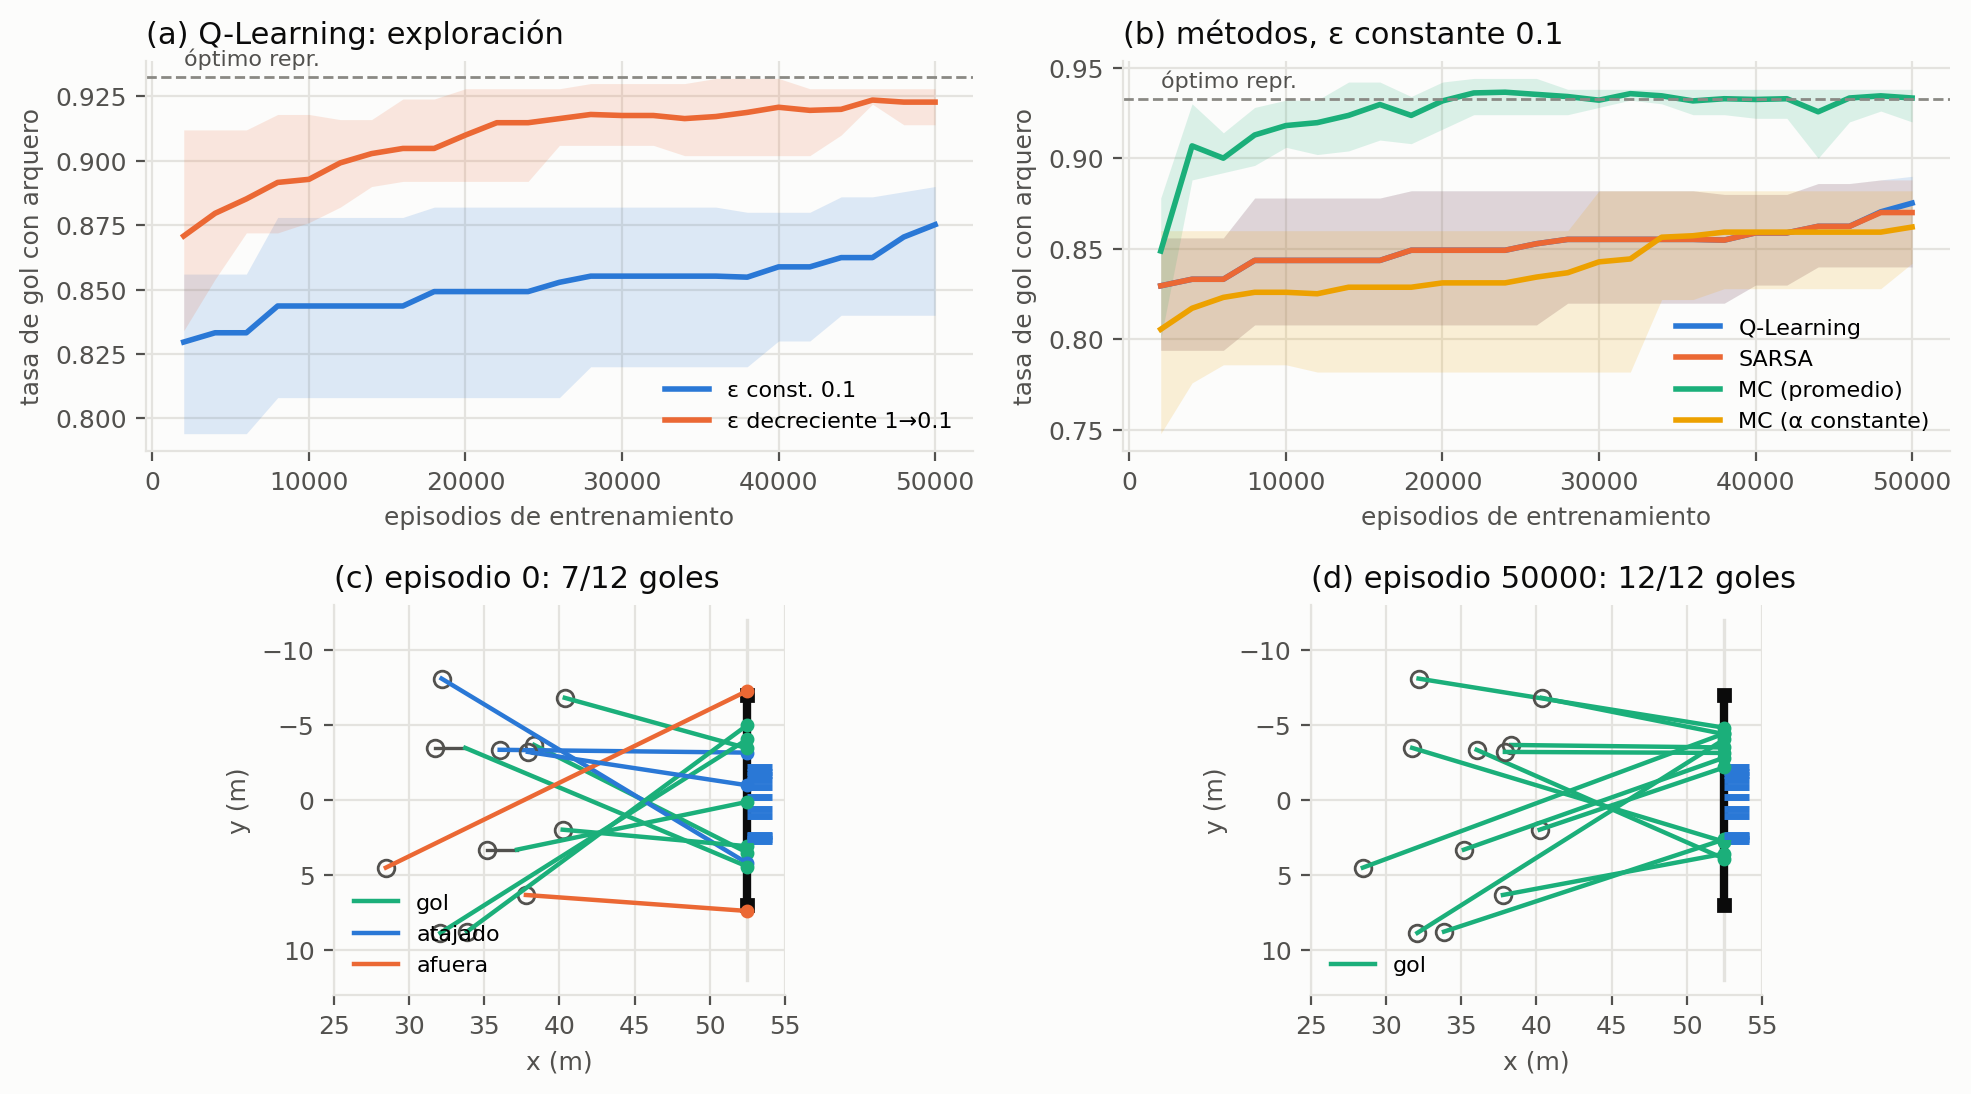
\includegraphics[width=0.88\textwidth]{fig_report_shooting.png}
    \caption{Tiro a puerta, con arquero. (a) Ablación de exploración de Q-Learning; (b) los cuatro métodos con
    $\varepsilon$ constante (Q-Learning queda bajo SARSA: sus curvas coinciden); media de 5 semillas, banda:
    mínimo--máximo. (c, d) Tiros greedy al inicio y al final del entrenamiento sobre 12 inicios (marca azul:
    arquero, que ataja a menos de 2\,m).}
    \label{fig:shoot}
\end{figure}

\subsection{Conducción}

Un controlador guionado (en posesión, girar hacia el arco y patear; si no, girar hacia el balón y correr) logra el
100\,\% en 20\,000 inicios (60.4 pasos en promedio, 85 como máximo), así que el 100\,\% es alcanzable. Q-Learning con
$\varepsilon$ decreciente llega al 97.7\,\% (media de las últimas 5 evaluaciones; Tabla~\ref{tab:ablall}). Aunque
el entorno es determinista, \textbf{la política greedy oscila} (Figura~\ref{fig:drib}a,b). Las caídas son timeouts:
un ciclo \texttt{TURN +35}/\texttt{TURN -35} entre dos estados agregados con valores casi empatados (41.87 frente a
42.00), que una actualización pequeña invierte. Con 245 estados (5 zonas de $d_b$ y 7 sectores de rumbo para balón y
arco) y el mismo presupuesto, Q-Learning y SARSA quedan en 100\,\% en cada una de las últimas 5 evaluaciones de las 5
semillas (Figura~\ref{fig:drib}c): \textbf{la oscilación viene de la agregación}, y 36 estados son pocos para esta
tarea.

\begin{figure}[!htb]
    \centering
    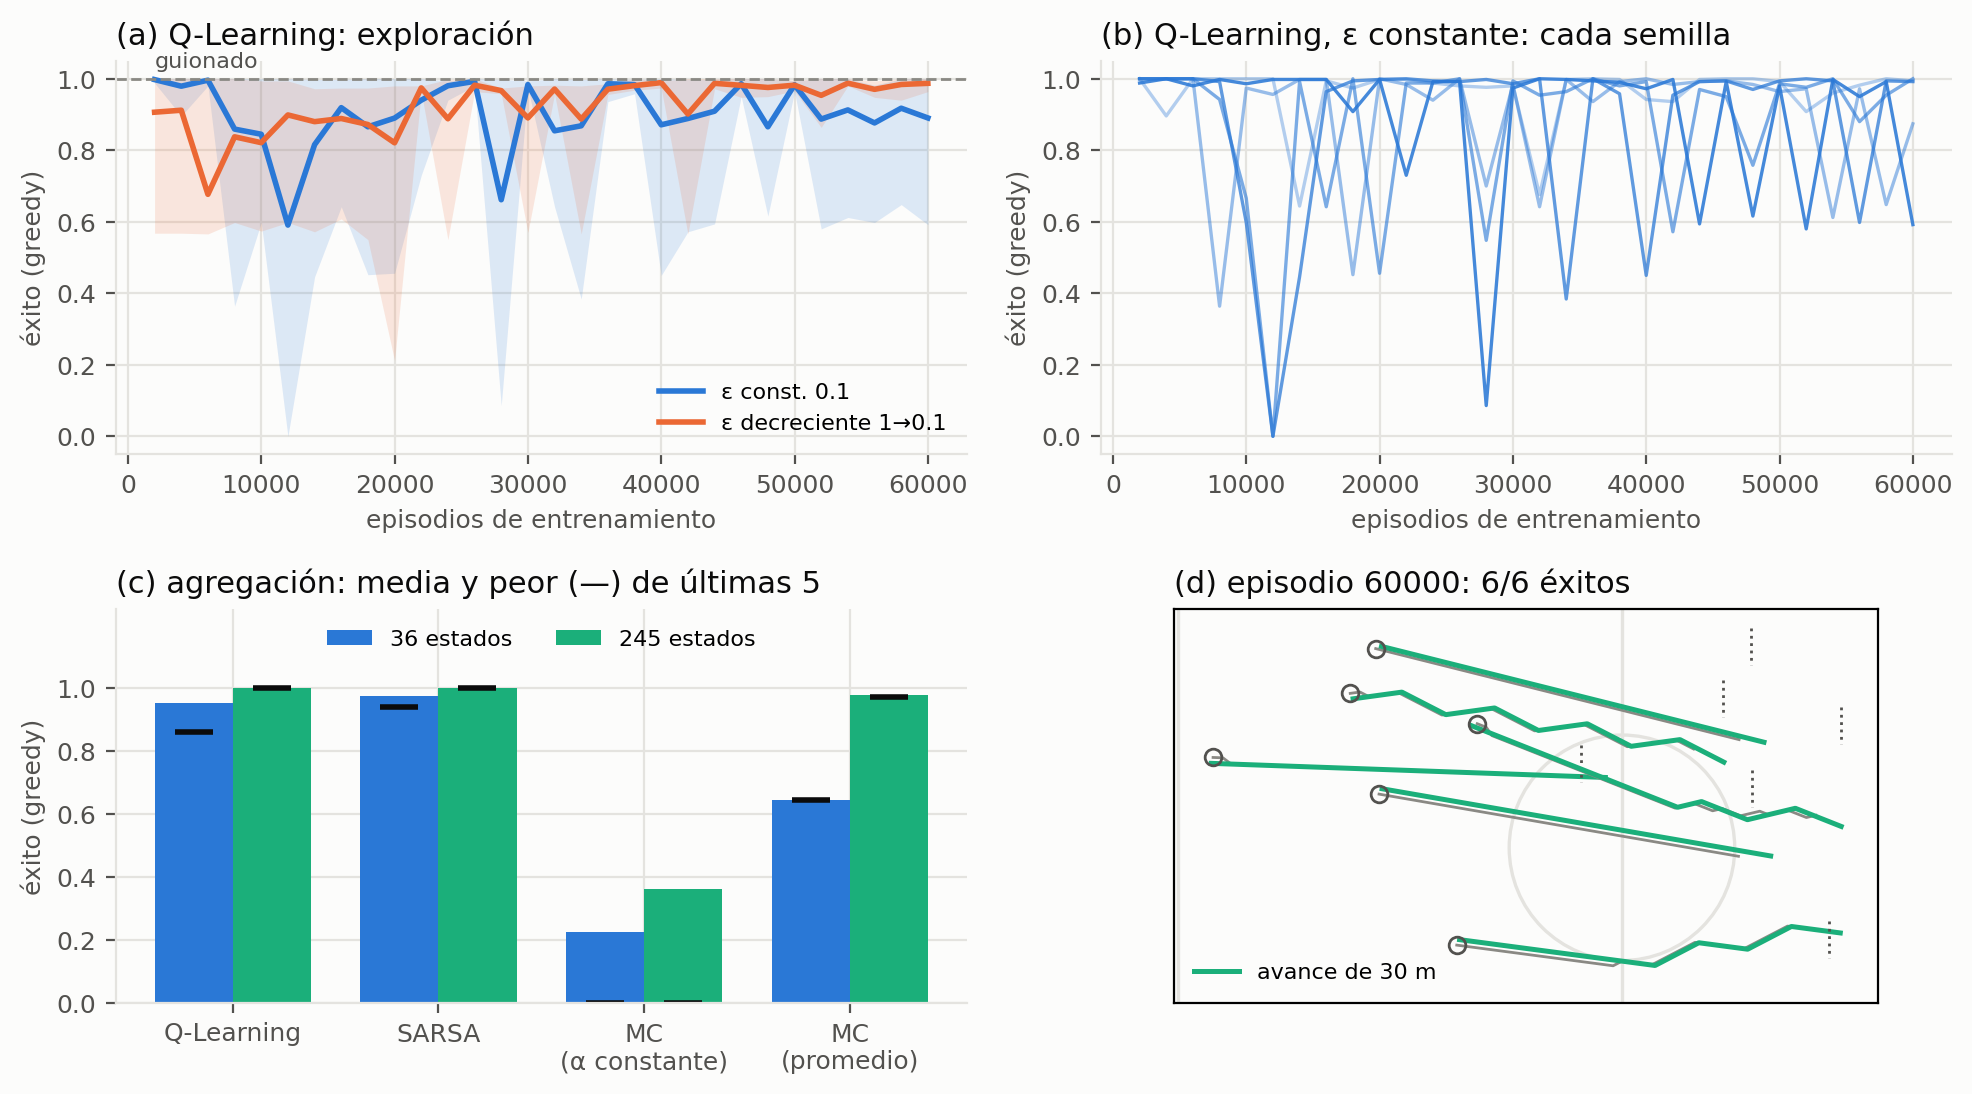
\includegraphics[width=0.88\textwidth]{fig_report_dribbling.png}
    \caption{Conducción. (a) Ablación de exploración de Q-Learning (media de 5 semillas, banda: mínimo--máximo);
    (b) cada semilla con $\varepsilon$ constante; (c) media (barra) y peor (marca) de las últimas 5 evaluaciones con
    36 y 245 estados (120\,000 episodios, $\varepsilon$ decreciente); (d) política greedy final de Q-Learning en 6
    inicios (verde: balón; gris: jugador; punteado: meta de 30\,m).}
    \label{fig:drib}
\end{figure}



\textbf{Verificación en \texttt{rcssserver}.} Ejecutamos la política final de la persecución en el servidor real,
200 episodios por distribución, con 0 comandos perdidos y 0 errores de reset: captura el \transkit{} con el reset
del kit (\transkitsim{} en nuestro simulador con física del servidor) y el \transunif{} en [5, 40]\,m
(\transunifsim). La verificación de tiro y conducción está en curso.

\section{Comparación de Métodos}
\label{sec:comp}

La Tabla~\ref{tab:comp} compara los cuatro métodos con $\varepsilon$ decreciente.

\begin{table}[htbp]
\centering\small
\begin{tabular}{@{}lcccc@{}}
\toprule
Tarea & Q-Learning & SARSA & MC (promedios) & MC ($\alpha$ constante) \\
\midrule
Persecución, [5, 40]\,m & \textbf{84.7} (77.0) & \textbf{85.3} (\textbf{83.3}) & \textbf{85.3} (\textbf{84.3}) & 45.8 (43.2) \\
Tiro, con arquero & \textbf{92.2} (90.9) & \textbf{92.2} (90.5) & \textbf{92.8} (\textbf{92.6}) & \textbf{91.8} (90.0) \\
Conducción, 36 estados & \textbf{97.7} (\textbf{92.4}) & \textbf{94.3} (76.2) & \textbf{90.4} (70.8) & 30.1 (22.3) \\
\bottomrule
\end{tabular}
\caption{Éxito greedy (\%): media de las últimas 5 evaluaciones y, entre paréntesis, AUC (éxito medio durante el
entrenamiento; mayor = aprende antes). Media de 5 semillas, $\varepsilon$ decreciente. En negrita, el mejor de cada
tarea y los que no se distinguen de él (IC 95\,\% solapados; los IC están en el notebook 13).}
\label{tab:comp}
\end{table}

\textbf{Por qué cada método rinde distinto en cada tarea.} Solo damos como causa lo que un experimento aisló:
\begin{itemize}
    \item \textbf{Persecución} (determinista, recompensa densa, sin riesgo): al final no hay diferencia entre
    Q-Learning, SARSA y MC con promedios; el techo lo pone la representación (óptimo 87.9\,\%). SARSA y MC aprenden
    antes; no aislamos por qué.
    \item \textbf{Tiro} (casi una decisión, resultado estocástico y terminal): Q-Learning y SARSA son idénticos por
    construcción, porque solo difieren al hacer bootstrap y el tiro termina el episodio. MC con promedios aprende
    antes y es el único que no se retrasa con $\varepsilon$ constante (93.2\,\% frente a 86.0--86.6\,\%). Causa
    aislada: con $Q_0 = 0$ y valores reales de 70--100, un paso $\alpha = 0.03$ corrige lento las acciones poco
    visitadas ($\max_a Q$ subestima $V^*$ en 6.6 puntos), mientras que el paso $1/N$ fija $Q$ en el primer retorno y
    luego da la media muestral de un resultado estacionario; $\alpha = 0.1$, $Q_0 = 100$ o 4 veces más episodios
    cierran la brecha. El sesgo de maximización que predijimos para Q-Learning no apareció: el $\max$ casi no
    interviene, porque solo entra tras \texttt{CONDUCIR}.
    \item \textbf{Conducción} (determinista, $\sim$60 pasos, estados agregados): al final Q-Learning, SARSA y MC con
    promedios no se distinguen (el IC de MC es muy ancho, 79--99\,\%), pero \textbf{Q-Learning aprende mucho antes}
    (AUC 92.4 frente a 76.2 y 70.8): mientras $\varepsilon$ es alto, SARSA y MC estiman el valor de una política casi
    aleatoria y Q-Learning, off-policy, ya aprende la greedy (con 245 estados está en 100\,\% desde la primera
    evaluación). Con $\varepsilon$ constante SARSA es el más estable (96.8 frente a 89.7\,\%), aunque parte puede
    venir de $\alpha$ (0.03 frente a 0.1). Dos predicciones fallaron: no hay ``acantilado'' que haga a SARSA más
    prudente (los métodos TD pierden el balón en $\le 0.5$\,\% de los episodios de entrenamiento, y con radio de
    pérdida de 8\,m nada cambia), y MC no resistió mejor la agregación~\cite{singh1994}: con 36 estados congela su
    política en algunas semillas (64.5\,\% con 120\,000 episodios) y con 245 llega a 97.8\,\%.
    \item \textbf{MC con $\alpha$ constante} falla en las dos tareas de episodios largos, también con 245 estados y
    $\alpha$ de hasta 0.003, y funciona en el tiro, de un paso. No aislamos la causa.
\end{itemize}

\section{Discusión}
\label{sec:disc}

\textbf{Exploración.} El efecto de $\varepsilon$ decreciente depende de la tarea y de $\alpha$. En la persecución
aprende antes (70\,\% en 12\,000 episodios frente a 16\,000) y termina algo más alto. En el tiro termina más alto con
$\alpha = 0.03$, pero es solo velocidad: la brecha desaparece con $\alpha = 0.1$, $Q_0 = 100$ o más episodios, y
elegir $\alpha$ solo con $\varepsilon$ decreciente favoreció a este en la comparación. En la conducción, con $\alpha$
elegido para cada exploración, termina mejor en Q-Learning, aunque $\varepsilon$ constante aprende antes (su retorno
de entrenamiento se estabiliza en $\approx 3\,000$ episodios frente a $\approx 35\,000$); en SARSA no hay diferencia
final.

\textbf{Discretización.} Fue el factor que más pesó. En la persecución, la discretización del kit (20 estados) llega
al 56.6\,\%, nuestra primera versión (20) al 61.0\,\%, R3 (99) al 84.7\,\% y R4 (150) cae al 81.0\,\% por falta de
datos; en la conducción, pasar de 36 a 245 estados elimina la oscilación.

\textbf{\textquestiondown{}Por qué no mejores resultados en la persecución?} En [5, 40]\,m: (i) 40 pasos no alcanzan
para los inicios lejanos (el óptimo captura el 18.7\,\% a 35--40\,m), así que el 90\,\% no es alcanzable con ningún
algoritmo; (ii) la tabla deja una brecha pequeña con el óptimo, a 30--40\,m; (iii) la física del kit no es la del
servidor (aceleración gradual, giros que dependen de la velocidad, ruido, visión parcial), por eso transfiere mal. Una
política entrenada con la física del servidor alcanza el 73.5\,\% $\pm$ 3.1 en vivo, sin errores de socket en 500
episodios consecutivos.

\section{Conclusiones}

\begin{itemize}
    \item \textbf{Criterios:} persecución, 100\,\% con el reset del kit (en [5, 40]\,m el 90\,\% no es alcanzable:
    óptimo 87.9\,\%, nuestro 85.7\,\%); tiro, 100\,\% sin arquero y 92.3\,\% con arquero (óptimo de la
    representación: 93.3\,\%); conducción, 97.7\,\% (100\,\% con 245 estados).
    \item \textbf{Modelado:} las cotas exactas o constructivas separan los límites de la tarea de los del
    aprendizaje; la representación pesó más que el algoritmo.
    \item \textbf{Métodos:} ninguno gana en todas las tareas. MC con promedios fue el mejor en el tiro (un paso,
    resultado estocástico); en la conducción Q-Learning aprendió antes y SARSA fue el más estable con $\varepsilon$
    constante; MC con $\alpha$ constante falló en las dos tareas de episodios largos. Son resultados de tres tareas,
    no reglas generales. $\varepsilon$ decreciente nunca terminó peor de forma detectable, pero su ventaja depende
    de $\alpha$.
    \item \textbf{Pendiente para P1:} cooperación 2v1 y la verificación en \texttt{rcssserver} de tiro y conducción.
    Para P2: aproximadores continuos (DQN/PPO), que evitan elegir a mano la agregación, y entrenar con la física del
    servidor.
\end{itemize}

\begin{thebibliography}{9}
\bibitem{sutton}
R. S. Sutton and A. G. Barto, \textit{Reinforcement Learning: An Introduction}, 2nd ed., MIT Press, 2018.
\bibitem{robocup}
H. Kitano et al., ``The RoboCup Soccer Server,'' in \textit{RoboCup-97: Robot Soccer World Cup I}, Springer, 1998, pp. 62--79.
\bibitem{rcssmanual}
M. Chen et al., \textit{Users Manual: RoboCup Soccer Server}, RoboCup Federation, 2003.
\bibitem{watkins1992}
C. J. C. H. Watkins and P. Dayan, ``Q-learning,'' \textit{Machine Learning}, vol. 8, pp. 279--292, 1992.
\bibitem{pardo2018}
F. Pardo, A. Tavakoli, V. Levdik, and P. Kormushev, ``Time limits in reinforcement learning,'' in \textit{ICML}, 2018, pp. 4045--4054.
\bibitem{singh1994}
S. P. Singh, T. Jaakkola, and M. I. Jordan, ``Learning without state-estimation in partially observable Markovian decision processes,'' in \textit{ICML}, 1994, pp. 284--292.
\end{thebibliography}

\end{document}
